
\documentclass{ieeeaccess}
\usepackage{cite}
\usepackage{amsmath,amssymb,amsfonts}
\usepackage{algorithmic}
\usepackage{graphicx}
\usepackage{textcomp}
\def\BibTeX{{\rm B\kern-.05em{\sc i\kern-.025em b}\kern-.08em
    T\kern-.1667em\lower.7ex\hbox{E}\kern-.125emX}}


\begin{document}
\history{Date of publication 2024 10.}
\doi{10.1109/ACCESS.2017.DOI}

\title{DRG prediction}
\author{\uppercase{Cristián Ormazábal}\authorrefmark{1}}
\address[1]{Ormasoft EIRL (e-mail: cristian@ormasoft.cl)}
\address[2]{Candidate to Master of computing (e-mail: c.ormazabalortega@uandresbello.edu)}

\begin{abstract}
This study focuses on the analysis of a dataset from El Pino Hospital, which contains detailed information on diagnoses (D01-D35) and procedures (P01-P30) associated with patients, along with demographic data such as age, sex, the diagnosis-related group (DRG), and an additional diagnostic classification that we created by selecting the first two digits of the DRG column. The main objective is to apply data analysis and machine learning techniques to identify relevant patterns within the diagnoses and procedures, aiming to improve accuracy in their classification and prediction.
\end{abstract}

\titlepgskip=-15pt

\maketitle

\section{Introduction}
\label{sec:introduction}
\PARstart{I}{n} the hospital setting, the efficient management of diagnoses and medical procedures is crucial to optimize resources, improve the quality of care, and reduce operational costs. One of the most commonly used methodologies for grouping diagnoses and managing resources is the Diagnosis-Related Groups (DRG) system, which classifies patients based on their clinical conditions and the medical procedures performed. This system facilitates cost forecasting and clinical outcome analysis, while also standardizing the treatment of complex cases.

This study focuses on the analysis of a dataset from El Pino Hospital, which contains detailed information on diagnoses (D01-D35) and procedures (P01-P30) associated with patients, along with demographic data such as age, sex, the diagnosis-related group (DRG), and an additional diagnostic classification that we created by selecting the first two digits of the DRG column. The main objective is to apply data analysis and machine learning techniques to identify relevant patterns within the diagnoses and procedures, aiming to improve accuracy in their classification and prediction.

Through this analysis, the goal is not only to explore the data's behavior using descriptive statistics but also to develop a predictive model that supports medical decision-making, thereby optimizing resource allocation and improving the quality of hospital services.

\section{Objective}
\label{sec:objective}
The main objective of this study is to analyze and model the diagnoses and medical procedures of El Pino Hospital using data analysis and machine learning techniques. The aim is to identify patterns in the data that can improve the classification of diagnoses and procedures, optimize hospital management, and support clinical decision-making. Specifically, the goal is to develop a predictive model based on Diagnosis-Related Groups (DRG) and other relevant variables, which helps forecast patient outcomes in terms of treatments, costs, and clinical results, thereby contributing to improved quality of medical care and operational efficiency at the hospital.

\section{Methodology}
\label{sec:methodology}
The study will be conducted using a data analysis approach and advanced machine learning techniques. First, the dataset will undergo cleaning and exploration to ensure data quality by identifying potential outliers, missing data, and relevant features. Subsequently, a predictive model will be implemented using Recurrent Neural Networks (RNN), as these are particularly well-suited for handling sequential data like that found in hospital records. RNNs will allow for capturing dependencies between diagnoses and procedures, improving the model's predictive capabilities. Additionally, feature engineering techniques will be applied to optimize the model's performance, and metrics such as precision, recall, and F1-score will be evaluated to select the most appropriate model. The implementation will be carried out in a machine learning environment, ensuring the model's replicability and scalability for use in future hospital studies.

\section{Experiments}
\label{sec:experiments}

\begin{figure}
    \centering
    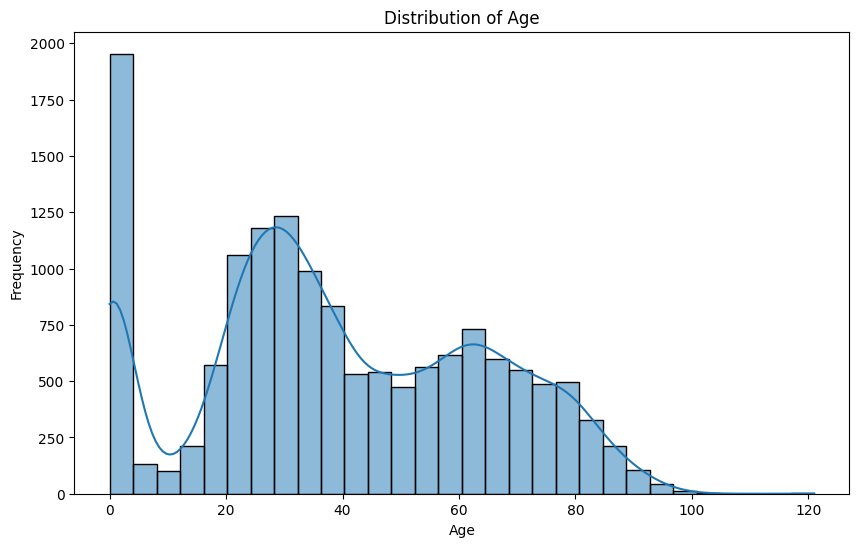
\includegraphics[width=0.5\linewidth]{image2.png}
    \caption{Distribution of age}
    \label{fig:enter-label}
\end{figure}

\begin{figure}
    \centering
    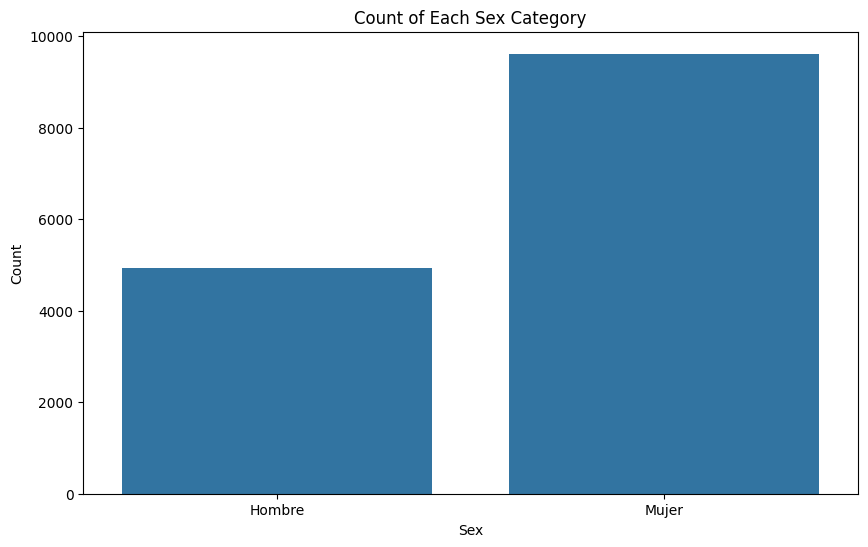
\includegraphics[width=0.5\linewidth]{image.png}
    \caption{Count of each sex category}
    \label{fig:enter-label}
\end{figure}

\begin{figure}
    \centering
    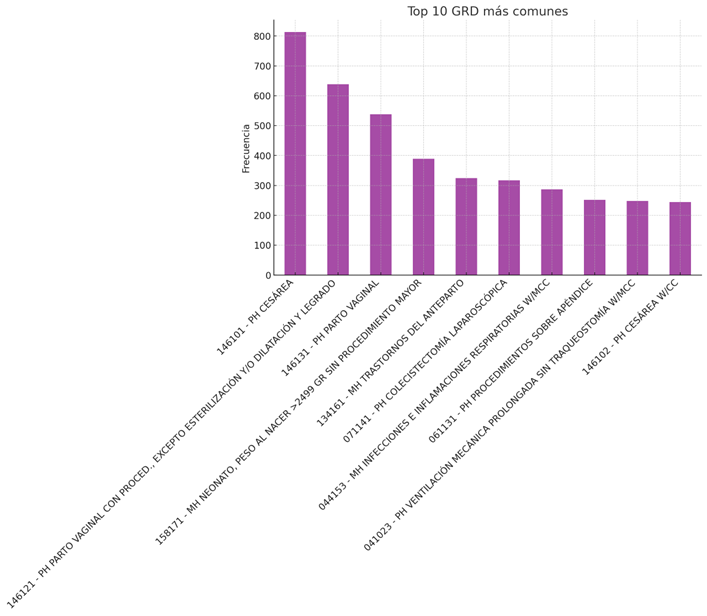
\includegraphics[width=0.5\linewidth]{image3.png}
    \caption{Most common DRG}
    \label{fig:enter-label}
\end{figure}

\begin{figure}
    \centering
    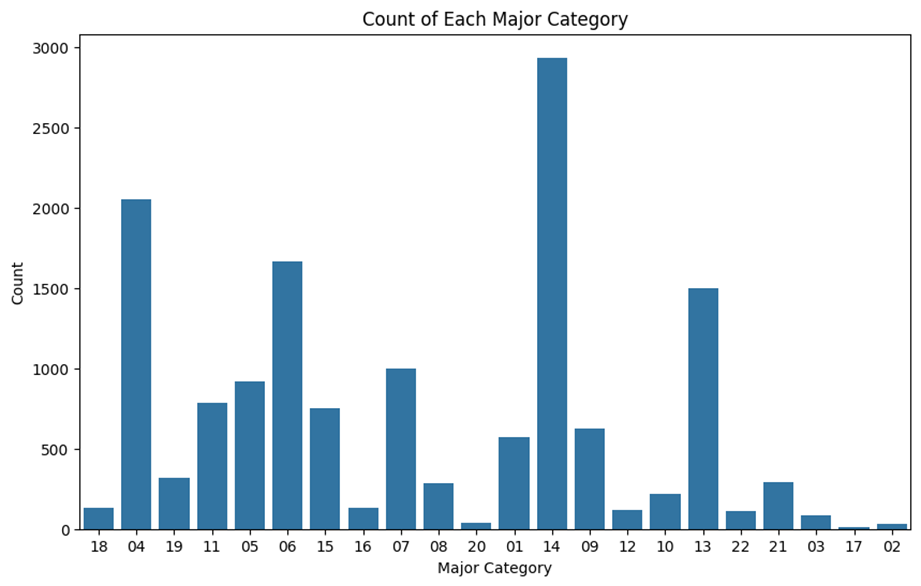
\includegraphics[width=0.5\linewidth]{image4.png}
    \caption{Count of each major category}
    \label{fig:enter-label}
\end{figure}

There are some categories with very few data points, and these will be candidates for running the model with all categories compared to removing the minority ones, in order to verify which model produces better results. The same approach will be applied to the age distribution, as there are many cases for younger individuals (around the first year of life), and potentially the diagnoses in this age group will be different, so we may also need to divide the data accordingly.

To achieve this, the texts of the diagnostics and procedures will be converted to embeddings and the embeddings padded in a single value in the 'all\_text' column.

Then, the RNN will be calculated using the all\_text+Age+Sex+CLASS vs the DRG column.

With this and some experimentation with the parameters, we get the following (figure 5):

\begin{figure}
    \centering
    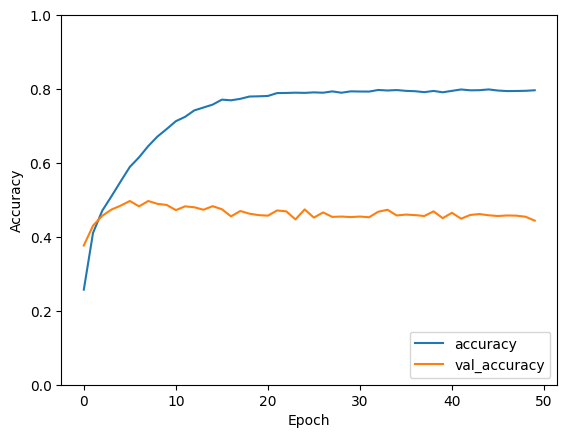
\includegraphics[width=0.5\linewidth]{image5.png}
    \caption{Validation of the RNN model for Age > 1}
    \label{fig:enter-label}
\end{figure}

\section{Conclusion}
\label{sec:conclusion}
Using text embeddings helps achieve a faily good model, with accuracy close to 80%.
We tested separately for Age > 1.


For Age < 1 we get (figure 6):

\begin{figure}
    \centering
    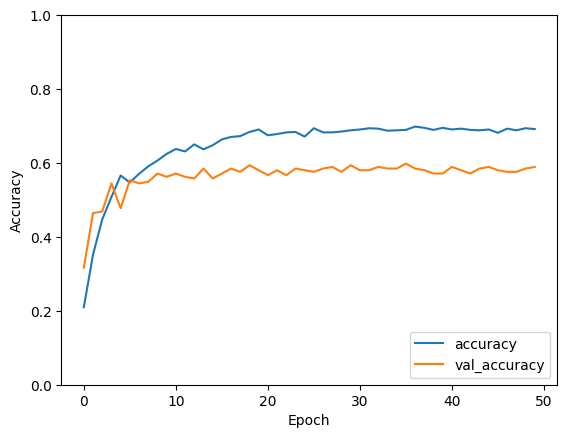
\includegraphics[width=0.5\linewidth]{image6.png}
    \caption{Model performance for Age < 1}
    \label{fig:enter-label}
\end{figure}

Separating different models by Sex didn't improve the resulting model.


\begin{thebibliography}{99}

\bibitem{shickel2017deep}
B. Shickel, P. J. Tighe, A. Bihorac, and P. Rashidi, ``Deep EHR: A survey of recent advances on deep learning techniques for electronic health record (EHR) analysis,'' \textit{IEEE Journal of Biomedical and Health Informatics}, vol. 22, no. 5, pp. 1589--1604, 2017.

\bibitem{rajkomar2019machine}
A. Rajkomar, J. Dean, and I. Kohane, ``Machine learning in medicine,'' \textit{New England Journal of Medicine}, vol. 380, no. 14, pp. 1347--1358, 2019.

\bibitem{saberzadeh2020development}
B. Saberzadeh-Ardestani, A. Rezapour, Z. Kavosi, and M. A. Abbasi-Moghadam, ``Development and evaluation of a case-mix prediction model for hospital resource consumption based on diagnosis-related groups (DRG),'' \textit{Frontiers in Public Health}, vol. 8, p. 401, 2020.

\bibitem{zhou2016defining}
S. M. Zhou, F. Fernandez-Gutierrez, J. Kennedy, R. Cooksey, M. Atkinson, S. Denaxas, et al., ``Defining disease phenotypes using national linked electronic health records: A case study of type 2 diabetes mellitus,'' \textit{Journal of Biomedical Informatics}, vol. 64, pp. 37--43, 2016.

\bibitem{rosner2015fundamentals}
B. Rosner, \textit{Fundamentals of Biostatistics}, 7th ed., Cengage Learning, 2015.

\bibitem{altman1990practical}
D. G. Altman, \textit{Practical Statistics for Medical Research}, Chapman & Hall/CRC, 1990.

\end{thebibliography}



\EOD

\end{document}
